\documentclass[10pt, a4paper, italian]{article}
\usepackage[T1]{fontenc}
\usepackage[utf8]{inputenc}
\usepackage{amsmath, amssymb, amsthm, thmtools, amsfonts, mathtools}
\usepackage{nicefrac}
\usepackage{calc}
\usepackage[pdftex, hyperindex, plainpages=false]{hyperref}
\usepackage[nameinlink]{cleveref} %load before classicthesis (clash)
%\usepackage[nochapters,pdfspacing]{classicthesis}
\usepackage{siunitx}
\usepackage[siunitx]{circuitikz}

\usepackage[a4paper]{geometry}
\usepackage{float}
\usepackage{mdframed}
\usepackage{titling}
\usepackage{booktabs}
\usepackage{graphicx}
\usepackage{caption, subcaption}
\usepackage{xcolor}
\usepackage[italian]{babel}
\usepackage{pgfplots}
\usepackage{listings}
%\usepackage{lmodern}
\usepackage{url}
\usepackage{enumitem}
\usepackage{tikz} %loads after classicthesis (xcolor incompat)

% lets graphicx know path where figures to be included are found
\graphicspath{{../figs/}}
\makeatletter
\def\input@path{{../figs/}}
%or: \def\input@path{{/path/to/folder/}{/path/to/other/folder/}}
\makeatother

% tikz pgf plots setup
\usepgfplotslibrary{external}
\pgfplotsset{compat=1.15}
%\tikzexternalize

% spaces and significant digits/figures for measurements
\sisetup{free-standing-units, space-before-unit, number-unit-product = \;,
scientific-notation = false, round-mode = figures, round-precision = 1,}

% turns all (hyperlinked) references black [default is blue]
\hypersetup{
	linktoc=all,
	colorlinks=true,
	linkcolor=black
}

% code listings config
%\lstset{
%language=Python,
%basicstyle=\ttfamily,
%columns=fullflexible,
%keepspaces=true,
%}

% mdframed (for boxed text) configuration
\mdfsetup{linewidth=0.6pt}

% Default fixed font does not support bold face
\DeclareFixedFont{\ttb}{T1}{txtt}{bx}{n}{12} % for bold
\DeclareFixedFont{\ttm}{T1}{txtt}{m}{n}{12}  % for normal

% Custom colors
\usepackage{color}
\definecolor{deepblue}{rgb}{0,0,0.5}
\definecolor{deepred}{rgb}{0.6,0,0}
\definecolor{deepgreen}{rgb}{0,0.5,0}

% Commands 
\newcommand{\executeiffilenewer}[3]{%
	\ifnum\pdfstrcmp{\pdffilemoddate{#1}}%
		{\pdffilemoddate{#2}}>0%
	{\immediate\write18{#3}}\fi%
}
% input .svg --> .pdf_tex graphs
%\newcommand{\includesvg}[1]{%
%	\executeiffilenewer{#1.svg}{#1.pdf}%
%	{inkscape -z -D --file=#1.svg %
%	--export-pdf=#1.pdf --export-latex}%
%	\input{#1.pdf_tex}%
%}
% Thanks UniPi's Department of Physics E. Fermi
\newcommand{\thanksdf}{(\thanks{Dipartimento di Fisica E.~Fermi,%
Universit\`a di Pisa - Pisa, Italy.}\;)}

% hyperlink to email address
\newcommand{\mail}[1]{\href{mailto:#1}{\textsf{#1}}}

% \vec for bold vectors, instead of overarrows (now "\arrvec")
\let\arrvec=\vec
\renewcommand{\vec}[1]{\boldsymbol #1}
% replaces straight phi with slanted phi
\renewcommand{\phi}{\varphi}
% replaces straight eps with curved epsilon
\newcommand{\eps}{\varepsilon}
% abbreviation for (sub_/super^)scripts of \lim, \sum,... in inline math
\newcommand{\ds}{\displaystyle}

% blackboard/number set letters
\newcommand{\CC}{\mathbb C}
\newcommand{\HH}{\mathbb H}
\newcommand{\KK}{\mathbb K}
\newcommand{\NN}{\mathbb N}
\newcommand{\PP}{\mathbb P}
\newcommand{\QQ}{\mathbb Q}
\newcommand{\RR}{\mathbb R}
\newcommand{\ZZ}{\mathbb Z}

\newcommand{\Abs}[1]{{\left\Vert #1\right\Vert}}
\newcommand{\enclose}[1]{{\left( #1 \right)}}
\newcommand{\Enclose}[1]{{\left[ #1 \right]}}
\newcommand{\floor}[1]{\left\lfloor #1 \right\rfloor}
\newcommand{\ceil}[1]{\left\lceil #1 \right\rceil}
\newcommand{\To}{\rightrightarrows}

% Math operators
\DeclareMathOperator{\divergence}{div}
\renewcommand{\div}{\divergence}
\DeclareMathOperator{\Imaginarypart}{Im}
\renewcommand{\Im}{\Imaginarypart}
\DeclareMathOperator{\Realpart}{Re}
\renewcommand{\Re}{\Realpart}
%\DeclareMathOperator{\arg}{arg}
\DeclareMathOperator{\tg}{tg}
\DeclareMathOperator{\arctg}{arctg}
\DeclareMathOperator{\settsinh}{settsinh}
\DeclareMathOperator{\settcosh}{settcosh}
\DeclareMathOperator{\tr}{tr}
\DeclareMathOperator{\im}{im}
\DeclareMathOperator{\sgn}{sgn}
\DeclareMathOperator{\diag}{diag}

\DeclarePairedDelimiter{\norm}{\lVert}{\rVert}
\DeclarePairedDelimiter{\scalar}{\langle}{\rangle}

% Logarithm with arbitrary base.
% -> log_10
\newcommand{\llog}[1][10]{\log_{#1}}

% Absolute value.
% -> |x|
\newcommand{\abs}[1]{\left| #1 \right|}

% Powers.
% -> x^a
\newcommand{\power}[2][2]{\left( #2 \right)^{#1}}

% Square.
% -> x^2
\newcommand{\sq}[1]{\power[2]{#1}}

% Expansion of the binomial coefficient.
% -> n1!/(n2!(n1 - n2)!)
\newcommand{\binomexpr}[2]{\frac{#1!}{#2!(#1 - #2)!}}

% Expression evaluation at a given point with square brackets.
% -> [x]_{a}
\newcommand{\at}[2]{\left[ #1\right]_{\makebox[-1pt][l]{${\scriptstyle#2}$}}}

% Expression evaluation in an interval.
% -> [x] _{a}^{b}
\newcommand{\eval}[3]{\left.#1%
  \right|_{\makebox[-1pt][l]{${\scriptstyle#2}$}}^{\makebox[-1pt][l]{${\scriptstyle#3}$}}}

% Upright d in math mode (for differentials).
% -> d
\newcommand{\ud}{\mathrm{d}}

% Differential.
% -> dx
\newcommand{\diff}[1][x]{\,\ud{#1}}

% Base command for defining derivatives.
% -> df/dx or d^kf/dx^k
\newcommand{\basederivative}[4][]{%
  \displaystyle%
  \ifx\\#1\\\frac{#4#2}{#4#3}%
  \else%
  \frac{#4^#1#2}{#4#3^#1}%
  \fi%
}

% Total derivative.
% -> df/dx(x) or d^kf/dx^k(x)
\newcommand{\td}[4][]{%
  \basederivative[#1]{#2}{#3}{\ud}%
  \ifx\\#4\\%
  \else%
  \mkern-4mu\left(#4\right)%
  \fi%
}

% Partial derivative.
% -> df/dx(x) or d^kf/dx^k(x)
\newcommand{\pd}[4][]{%
  \basederivative[#1]{#2}{#3}{\partial}%
  \ifx\\#4\\%
  \else%
  \mkern-4mu\left(#4\right)%
  \fi%
}

\newcommand{\intinf}{\int_{-\infty}^{\infty}\!\!\!}

\newcommand{\cinterval}[2]{\left[\, #1,~#2 \,\right]}

\newcommand{\linterval}[2]{\left[\, #1,~#2 \,\right)}

\newcommand{\rinterval}[2]{\left(\, #1,~#2 \,\right]}

\newcommand{\ointerval}[2]{\left(\, #1,~#2 \,\right)}

\newcommand{\prob}[1]{\displaystyle P\left(#1\right)}

\newcommand{\pvalue}{\emph{$p$-value}}

\newcommand{\cond}{\,|\,}

\newcommand{\expect}[1]{\displaystyle E\left[#1\right]}

\newcommand{\mom}[2][]{\displaystyle {\cal M}_{#2}\ifx\\#1\\\else(#1)\fi}

\newcommand{\momalg}[1]{\displaystyle \lambda_{#1}}

\newcommand{\momcen}[1]{\displaystyle \mu_{#1}}

\newcommand{\skewness}{\displaystyle \gamma_1}

\newcommand{\kurtosis}{\displaystyle \gamma_2}

\newcommand{\charf}[1][x]{\phi_{#1}}

\newcommand{\momgenf}[1][x]{M_{#1}}

\newcommand{\fwhm}{{\scriptstyle \textsc{FWHM}}}

\newcommand{\hwhm}{{\scriptstyle \textsc{HWHM}}}

\newcommand{\median}{\mu_{\nicefrac{1}{2}}}

\newcommand{\var}[1]{\ensuremath{\text{Var}\left(#1\right)}}

\newcommand{\cov}[2]{\ensuremath{\text{Cov}\left(#1, #2\right)}}

\newcommand{\corr}[2]{\ensuremath{\text{Corr}\left(#1, #2\right)}}

\newcommand{\like}{\mathcal L}

\newcommand{\likelihood}[2][]{\like\ifx\\#2\\\else(#2\ifx\\#1\\\else;#1\fi)\fi}

\newcommand{\chisq}{\ensuremath{\chi^2}}

\newcommand{\chisquare}[2][]{\chisq\ifx\\#2\\\else(#2\ifx\\#1\\\else;#1\fi)\fi}

\newcommand{\loglikelihood}[2][]{\log\likelihood[#1]{#2}}

\newcommand{\pdf}[3][]{#2(#3\ifx\\#1\\\else;#1\fi)}

\newcommand{\binomialpdf}[2][]{\pdf[#1]{\mathcal B}{#2}}

\newcommand{\multinomialpdf}[2][]{\pdf[#1]{\mathcal M}{#2}}

\newcommand{\poissonpdf}[2][]{\pdf[#1]{\mathcal P}{#2}}

\newcommand{\uniformpdf}[2][]{\pdf[#1]{u}{#2}}

\newcommand{\exponentialpdf}[2][]{\pdf[#1]{\varepsilon}{#2}}

\newcommand{\gausspdf}[2][]{\pdf[#1]{N}{#2}}

\newcommand{\chisquarepdf}[2][]{\pdf[#1]{\wp}{#2}}

\newcommand{\cauchypdf}[2][]{\pdf[#1]{c}{#2}}

\newcommand{\erf}[1]{\ensuremath{\text{erf}\left(#1\right)}}

\newcommand{\dccases}[4][]{#2 \ifx\\#2\\\else=\fi %
  \begin{cases}
    \displaystyle #3 & \text{per variabili discrete}\\
    \displaystyle #4 & \text{per variabili continue}#1
  \end{cases}
}
% sub/super-scriptable for all symbol as math operator 
\newcommand\Scaleforall[1]{\vcenter{\hbox{\scalefont{#1}$\forall$}}}

\DeclareMathOperator*\forevery{%
  \vphantom\sum
  \mathchoice{\Scaleforall{2}}{\Scaleforall{1.4}}{\Scaleforall{1}}{\Scaleforall{0.75}}}
\usepackage{multicol}
\geometry{left=2cm, right=2cm, top=2cm, bottom=2cm}
\usepackage{colortbl}
\usepackage{diagbox}
\usepackage{tkz-graph}
\usetikzlibrary{automata, positioning, arrows}
\newenvironment{FSM}{
\begin{tikzpicture}
\tikzset{
->, % makes the edges directed
>=stealth', % makes the arrow heads bold
node distance=2cm, % specifies the minimum distance between two nodes. Change if necessary.
every state/.style={minimum size = 1cm, thick, fill=gray!10}, % sets the properties for each 'state' node
}
}{
\end{tikzpicture}
}

% indexes subsections with letters, sections with numbers (1.a, 1.b, ...)
\renewcommand{\thesubsection}{\thesection.\alph{subsection}}

% lets graphicx know path where figures to be included are found
\graphicspath{{../figs/}}

\author{Gruppo 1.AC \\ Matteo Rossi, Bernardo Tomelleri}
\title{EsD3: Macchine a stati finiti: semafori e riconoscitore di fronti}
\begin{document}
\date{\today}
\maketitle

\section{Misura componenti dei circuiti}
Riportiamo per completezza il valore della tensione continua di
alimentazione per i circuiti integrati misurata con il multimetro
\[
V_{CC} = 4.99 \pm 0.03 \si{\V}
\]

e il valore di capacità del condensatore di disaccoppiamento che collega le
linee di alimentazione a massa (sempre misurato con il multimetro)
\[
C_d = 97 \pm 4 \; \si{n\F}
\]

%=======================
\section{Implementazione di un semaforo con circuiti integrati}\label{sec: IC}
\subsection{Diagramma a stati del semaforo}
Nel caso di semaforo ``abilitato'' i possibili output sono 3 e abbiamo quindi deciso di implementarli con 3 stati interni della macchina; nel caso di semaforo ``disabilitato'' i possibili output sono 2, ma possono essere ottenuti riutilizzando due degli stati precedenti e l'input ``enable'' tramite un'opportuno circuito combinatorio (\texttt{FSM} di Mealy).

Si è deciso di codificare in due bit di memoria i tre stati $ (00) $, $ (01) $ e $ (10) $ che corrispondono, quando $ E = 1 $ (abilitato), ai tre output ``verde'', ``verde-giallo'', ``rosso'' (che si susseguono in modo ciclico). Quando invece $ E = 0 $ (disabilitato) vengono usati solamente $ (00) $ e $ (01) $, che corrispondono agli output del semaforo ``spento'' e ``giallo''.

\begin{figure}[htbp]
\centering
\begin{FSM}
\tikzset{
    LabelStyle/.style = {
        rectangle, rounded corners, draw,
        minimum width = 1em,
    },
    EdgeStyle/.append style = {-stealth}
}

   \node[state with output] (V) {$V/Y^0$ \nodepart{lower} $00$};
   \node[state with output, right of=V, xshift=2cm] (VG)
   {$VG/Y^1$ \nodepart{lower} $01$};
   \node[state with output, right of=VG, xshift=2cm] (R)
   {$R$ \nodepart{lower} $10$};
   
   \Edge[label = E](V)(VG)
   \Edge[label = E](VG)(R)

\tikzset{EdgeStyle/.append style = {-stealth, bend right = 30}}
   \Edge[label = D](VG)(V)
   \Edge[label = D](V)(VG)

\tikzset{EdgeStyle/.append style = {bend right = 50}}
   \Edge[label = E](R)(V)

\tikzset{EdgeStyle/.append style = {bend left = 50}}
   \Edge[label = D](R)(V)
\end{FSM}
\end{figure}

\subsection{Codifica degli stati della macchina}
La scelta della codifica in termini di bit \`e riassunta nella tabella che segue: $Q_0$ e $Q_1$ rappresentano rispettivamente lo stato delle uscite del primo e del secondo flip-flop e $S$ \`e lo stato associato.
\begin{table}[htbp]
	\centering
	\begin{tabular}{cc|cc}
	\toprule
	$S_E$ &	$S_D$ & $Q_0$ &	$Q_1$ \\
	\midrule
	\midrule
	$Y^-$ & $V$  & $0$	&	$0$	\\
	$Y^+$ & $VG$ & $0$	&	$1$	\\
	 	  & $R$  & $1$	&	$0$	\\
	\bottomrule
	\end{tabular}
	\caption{codifica binaria degli stati del semaforo. \label{tab:bit}}
\end{table}

\subsection{Tabelle di verità}
Si nota in particolare dal diagramma degli stati che il segnale di input ENABLE modifica l'output in maniera asincrona, mentre dalla tabella di verità (\cref{tab:2bit}) si può distinguere come lo stato futuro dipenda da quello precedente sfruttando la sincronia del segnale di clock per incrementare il contatore.

\begin{table}[htbp]
    \centering
    \begin{tabular}{c|c|cc|cc|c}
     \multicolumn{1}{c||}{ENABLE}&\multicolumn{1}{c}{ }&\multicolumn{2}{c||}{current state} &\multicolumn{2}{c}{next state}\\
     \hline
         && Q$_1$ & Q$_0$ & D$_1$ & D$_0$ & \\
         \hline
        1 & G & 0 & 0 & 0 & 1 & GY\\
       & GY & 0 & 1 & 1 & 0 & R\\
       & R & 1 & 0 & 0 & 0 & G\\
        & ... & 1 & 1 & X & X & ...\\
        \hline
        0 & OFF & 0 & 0 & 0 & 1 & Y \\
        & Y & 0 & 1 & 0 & 0 & OFF \\
         & OFF & 1 & 0 & 0 & 0& OFF \\
         &  ... & 1 & 1 & X & X & ...\\
    \end{tabular}
    \caption{Tabella di verità per il semaforo a 2 bit.}
    \label{tab:2bit}
\end{table}

Di conseguenza, è possibile associare agli output led G, Y, R una corrispondenza in termini di bit secondo la logica:
\begin{itemize}
    \item Q$_0$ = 1 $\longrightarrow$ led giallo acceso (Y)
    \item Q$_1$ = 0 (o equivalentemente: $\overline{Q_1}$ = 1) $\longrightarrow$ led verde acceso (G)
    \item Q$_1$ = 1 $\longrightarrow$ led rosso acceso (R)
\end{itemize}
tale logica è sempre sottomessa al segnale di ENABLE, che consente che i led verde e rosso si possano accendere effettivamente. \\

Questa codifica è quella sfruttata per la costruzione vera e propria del circuito collegando i led alle uscite dei Flip-Flop (ad esempio: led giallo in serie a Q$_0$). \\

Per la precisione, dal momento che l'accensione dei led verde e rosso è consentita solo quando ENABLE = 1, si possono utilizzare due porte AND per definire
\begin{itemize}
    \item $\overline{Q_1} \cdot E \longrightarrow$ led verde acceso (G)
    \item $Q_1 \cdot E \longrightarrow$ led rosso acceso (R)
\end{itemize}

\paragraph{AND-gate per led rosso}
Si potrebbe usare una porta AND per rendere l'attivazione del led rosso dipendente dal segnale di ENABLE. Da \cref{tab:2bit} infatti si nota che l'unica differenza di funzionamento si avrebbe durante la transizione di ENABLE: 1 $\rightarrow$ 0. In questo caso, lo spegnimento diventerebbe asincrono col segnale di clock anziché sincrono.

\subsection{Mappe di Karnaugh e logica combinatoria}
Le seguenti tabelle di Karnaugh aiutano a derivare le funzioni logiche degli stati futuri in dipendenza da quelli correnti: \\

\begin{minipage}{0.5\textwidth}
    \centering
    \begin{tabular}{c||c|c|c|c}
        \backslashbox{E}{Q$_1$Q$_0$} & 00 & 01 & 11 & 10\\
        \hline
        \hline
        0 & 0 & 0 & X & 0\\
        \hline
        1 & 0 & \cellcolor[HTML]{FF9999}1 & \cellcolor[HTML]{FF9999}X & 0\\
    \end{tabular}
    %\captionof{table}{Tabella di Karnaugh}
    \label{k1}\\
    \hfill \\
    $D_1=E \cdot Q_0$
\end{minipage}
\begin{minipage}{0.5\textwidth}
    \centering
    \begin{tabular}{c||c|c|c|c}
        \backslashbox{E}{Q$_1$Q$_0$} & 00 & 01 & 11 & 10\\
        \hline
        \hline
        0 & \cellcolor[HTML]{FF9999}1 & 0 & X & 0\\
        \hline
        1 & \cellcolor[HTML]{FF9999}1 & 0 & X & 0\\
    \end{tabular}
    %\captionof{table}{Tabella di Karnaugh}
    \label{k2}\\
   \hfill \\
    $D_0=\overline{Q_0}\cdot \overline{Q_1}$
\end{minipage}

\subsection{Costruzione del circuito}
Si è assemblato il circuito riportato in ~\cref{fig:semaforoSchema} e si
sono collegati i pin \texttt{preset} e \texttt{clear} dei D-FF a
$V_{CC}$ per evitare reset o clear spuri.
\begin{figure}[htbp]
    \centering
    \begin{circuitikz}
        \def\andScale{0.7};
        \def\cusu{-1};
        \def\mano{0.5}
        \def\yep{2}

        % componenti
        %% flip flop
        \draw (0,0) node[flipflop D] (ffSinistra) {};
        \draw (5,0) node[flipflop D] (ffDestra) {};

        %% and
        \node (andSinistra) at (-2, |- ffSinistra.pin 1) [and port, scale=\andScale] {};
        \node (andDestra) at (3, |- ffSinistra.pin 1) [and port, scale=\andScale] {};
        \node [and port, scale=\andScale] (andSopra) at (5,4) {};

        % per i crossing
        \node at ($ (ffSinistra.pin 4) + (\mano,0) $) (ancilla) {};

        %% led
        \node (G) at ($ (andSopra.out) + (3,0) $) {$ G $};
        \node (Y) at ($ (G) + (0,-0.5) $) {$ Y $};
        \node (R) at ($ (G) + (0,-1) $) {$ R $};

        % input
        \node (E) at ($ (andSopra.in 1) + (-9,0) $) {$ E $};
        \node (CLK) at ($ (E)+(0,-7) $) {\texttt{CLK}};

        % fili
        %% clock
        \draw (CLK) -| (ffDestra.pin 3);
        \draw (ffSinistra.pin 3) -- (ffSinistra.pin 3 |-, |- CLK);

        % and e ff
        \draw (andSinistra.out) -- (ffSinistra.pin 1);
        \draw (andDestra.out) -- (ffDestra.pin 1);
        \draw (E) -- (andSopra.in 1);
        \draw (ffSinistra.pin 4) -- ++ (\mano,0) |- (andSopra.in 2);
        \draw (andSinistra.in 2) -| (-3.5, |- E);
        \draw (andDestra.in 1) -- ($ (ffSinistra.pin 4 |-, |- andDestra.in 1) + (\mano,0) $);
        %% cacro del crossing pt 1
        \node at (ffSinistra.pin 4 |-, \yep) [jump crossing] (X1) {};
        \node at (ancilla |-, \yep) [jump crossing] (X2) {};
        \draw (andSinistra.in 1) |- (X1.west);
        \draw (X1.east) -- (X2.west);
        \draw (X2.east) -- (ffDestra.pin 6 |-, \yep);
        %% cancro del crossing pt 2
        \node at ($ (ffDestra.pin 3) + (0,\cusu) $) [jump crossing] (X) {};
        \draw (ffDestra.pin 4) |- (X.east);
        \draw (X.west) -| (andDestra.in 2);

        %% led
        \draw (andSopra.out) -- (G);
        \draw (ffDestra.pin 6) |- (Y);
        %% cancro del crossing
        \node at (ancilla |-, |- R) [jump crossing] (X1) {};
        \node at (ffDestra.pin 6 |-, |- R) [jump crossing] (X2) {};
        \draw (ffSinistra.pin 6) |- (X1.west);
        \draw (X1.east) -- (X2.west);
        \draw (X2.east) -- (R);

        % numeri dei pin
%        \draw (ffSinistra.pin 1) node[above] {2};
%        \draw (ffSinistra.pin 3) node[above] {3};
%        \draw (ffSinistra.pin 4) node[above] {6};
%        \draw (ffSinistra.pin 6) node[below] {5};
%
%        \draw (ffDestra.pin 1) node[above] {12};
%        \draw (ffDestra.pin 3) node[above] {11};
%        \draw (ffDestra.pin 4) node[above] {8};
%        \draw (ffDestra.pin 6) node[below] {9};
    \end{circuitikz}
    \caption{\label{fig:semaforoSchema}schema del semaforo Mealy con enable.}
\end{figure}

Per studiarne il comportamento generiamo nei due pin DIO 0 (CLOCK) e DIO 1
(ENABLE) dell'AD2 due segnali di clock di frequenza $f = \SI{20}{\hertz}$ e
$\SI{2}{\hertz}$ agli ingressi CLK ed $E$ del circuito. 

\subsection{Analisi e verifica del funzionamento del circuito}
\begin{figure}[htbp]
    \centering
    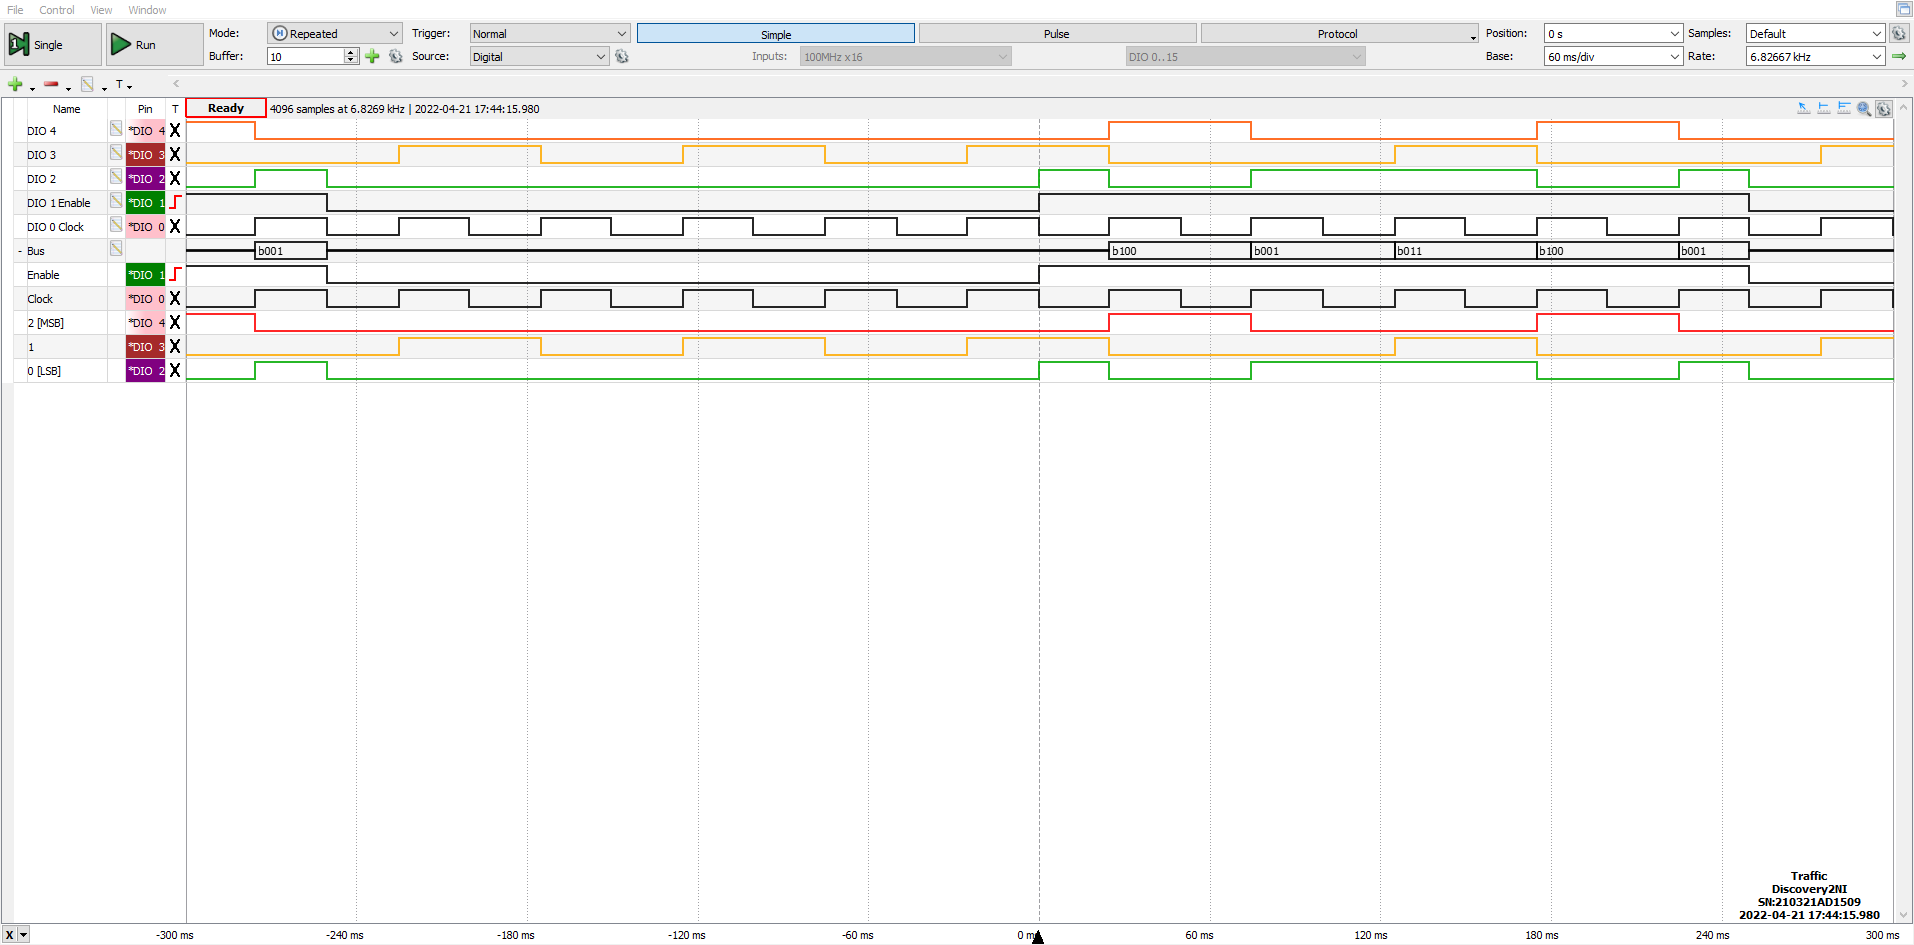
\includegraphics[width=\textwidth]{traffic}
    \caption{Acquisizione di un ciclo completo (frequenza 1 kHz) con Logic
    Analyzer dei segnali in ingresso e in uscita dal semaforo.
    \label{fig: dlatch}}
\end{figure}

%=======================
\section{Implementazione software della logica combinatoria con AD2/ROM}
\subsection{Costruzione del circuito}

\subsection{Implementazione delle tabelle di verità in ROM}

\subsection{Verifica del funzionamento del circuito}

\subsection{Variante svizzera del semaforo ROM}

%=======================
\section{Implementazione in software dei semafori con MCU (Arduino)}
Si vuole ricostruire il circuito precedente per il controllo di un semaforo tramite un microcontrollore (nel nostro caso utilizzeremo arduino); a questo scopo utilizzeremo come componenti uno switch, 3 led (rosso, verde e giallo) e una resistenza da $330 \ohm$ per limitare la corrente che scorre nei led.
\subsection{Collegamento LED semaforo alle uscite}

\subsection{Definizione interruttore di Enable}

\subsection{Implementazione del codice per la FSM}

\subsection{Versione svizzera del semaforo con Enable via Arduino}

%=======================
\section{Falling-edge detector}
\subsection{Progettazione FSM e costruzione dei circuiti}
Si vuole realizzare una FSM che riceve uno stream di bit su una linea di
ingresso e che accende un LED tutte le volte che si presenta un fronte di
discesa secondo il modello di Moore e secondo quello di Mealy.
\begin{figure}[htbp]
\centering
\begin{FSM}
\tikzset{node distance = 4cm, on grid, auto
}
\node (H) [state] {HIGH};
\node (C) [state, right of = H] {CHANGE};
\node (L) [state, right of = C] {LOW};
 
\path [-stealth, thick]
	(H) edge [loop left]  node {CLK=1}()
    (H) edge [bend left] node[above] {CLK=0} (C)
    (C) edge [bend left] node[above] {CLK=1} (H)
    (C) edge [bend left] node[above] {CLK=0} (L)
    (L) edge [bend left] node {CLK=1} (H)
    (L) edge [loop right]  node {CLK=0}();
\end{FSM}
\caption{Edge detector FSM di Moore
\label{diag: edgeMoore}}
\end{figure}

\begin{figure}[htbp]
\centering
\begin{FSM}
\tikzset{node distance = 4cm, on grid, auto
}
\node (H) [state] {HIGH};
\node (L) [state, right of = H] {LOW};
 
\path [-stealth, thick]
	(H) edge [loop left]  node {CLK=1}()
    (H) edge [bend left] node[above] {CLK=0, OUT=1} (L)
    (L) edge [bend left] node {CLK=1, OUT=0} (H)
    (L) edge [loop right]  node {CLK=0}();
\end{FSM}
\caption{Edge detector FSM di Mealy
\label{diag: edgeMealy}}
\end{figure}

\begin{table}[htbp]
	\centering
	\begin{tabular}{cc|cc}
	\toprule
	CLK & $Q$ & $Q^+$ &	OUT \\
	\midrule
	\midrule
	$0$  & $0$	&	$0$	& $0$ \\
	$0$  & $1$	&	$0$	& $1$ \\
	$1$  & $0$	&	$1$	& $0$ \\
	$1$  & $1$  & 	$1$ & $0$ \\
	\bottomrule
	\end{tabular}
	\caption{codifica binaria degli stati del detector di Mealy.
	$Q_+$ = CLK; OUT = $\overline{\text{CLK}} \cdot Q$
	\label{tab: bitMealy}}
\end{table}

\subsection{Definizione dello stream di bit casuali in ingresso}
Con la funzione Patterns di Waveform si invia un segnale di clock di
frequenza $f\ped{clk} = \SI{1}{k\Hz}$ al pin (CLK) del contatore e si
acquisiscono i segnali in uscita con la funzione Logic
dello stesso.

\subsection{Verifica del funzionamento e analisi della temporizzazione}


%=======================
\section*{Conclusioni e commenti finali}
Si è riusciti a verificare il corretto funzionamento di circuiti logici
sequenziali di crescente complessità e svariate applicazioni (e.g., sistemi di
controllo e misura) costruiti con porte NOT, NAND, XOR, D-Latch e contatori
sincroni.
In particolare sono stati realizzati e studiati un D-Latch, uno shift-register
con positive edge-triggered D-FF, un generatore di sequenze pseudocasuali e
alcuni tipi di divisore di frequenza con contatori binari.
Inoltre si è riusciti ad apprezzare l'effetto dei tempi di propagazione
delle porte sul loro comportamento, seppur in maniera limitata dalla bassa
risoluzione temporale dell'AD2.

%=======================
\section*{Dichiarazione}
I firmatari di questa relazione dichiarano che il contenuto della relazione \`e
originale, con misure effettuate dai membri del gruppo, e che tutti i firmatari
hanno contribuito alla elaborazione della relazione stessa.

\end{document}
